\documentclass{article}

% if you need to pass options to natbib, use, e.g.:
%     \PassOptionsToPackage{numbers, compress}{natbib}
% before loading neurips_2020

% ready for submission
% \usepackage{neurips_2020}

% to compile a preprint version, e.g., for submission to arXiv, add add the
% [preprint] option:
%     \usepackage[preprint]{neurips_2020}

% to compile a camera-ready version, add the [final] option, e.g.:
    \usepackage[final]{neurips_2020}


\usepackage[utf8]{inputenc} % allow utf-8 input
\usepackage[T1]{fontenc}    % use 8-bit T1 fonts
\usepackage{url}            % simple URL typesetting
\usepackage{booktabs}       % professional-quality tables
\usepackage{amsfonts, amsmath}       % blackboard math symbols
\usepackage{nicefrac}       % compact symbols for 1/2, etc.
\usepackage{microtype}      % microtypography
\usepackage{bbm}
\usepackage[colorlinks,
            linkcolor=blue,   
            anchorcolor=blue,
            citecolor=blue,
            ]{hyperref}
\usepackage{algorithm}
\usepackage{algorithmic}
\usepackage{palatino}
\usepackage[most]{tcolorbox}
\usepackage{listings} 


\newcommand{\x}{\mathbf{x}}
\newcommand{\R}{\mathbf{R}}
\numberwithin{equation}{section}
\numberwithin{figure}{section}

\title{Algorithms for Group Lasso}

\author{%
  Yihang Chen \\
  Department of Mathematics\\
  Peking University\\
  1700010780\\
}
\onecolumn

\begin{document}
\maketitle
\tableofcontents
\clearpage
\section{Problem formulation}

\begin{tcolorbox}[colback=blue!5!white,colframe=blue!75!black,title= Lasso]
Consider the $\ell_1$-regularized problem
\begin{equation}
    \min_x\quad f_\mu(x) = g(x)+\mu h(x):= \frac{1}{2}\|Ax-b\|_F^2+\mu\|x\|_{1,2} \label{eq:lasso}
\end{equation}
where $A\in \mathbb{R}^{m\times l},b\in \mathbb{R}^{n\times l}$ and $\mu>0$ are given.
\end{tcolorbox}

\section{Commercial Solvers}
We can obtain and solutions directly from cvx mosek and cvx gurobi. 

Denote $\hat{x}=\mathrm{vec}(x),\hat{b}=\mathrm{vec}(b)$, and $\hat{A}=\mathrm{diag}\underbrace{\{A, \cdots,A\}}_{l \times A}$. The indicator matrix of group $p$ is a diagnoal matrix whose $jj$-th element is defined as $1$ if $n|j-p$ and 0 otherwise.

The group lasso problem (\ref{eq:lasso}) is equivalent to the following cone optimization problem
\begin{equation}
\begin{split}
        \min&\quad  t+\mu \sum_{p=1}^n t_n\\
        \mathrm{s.t.}&\quad \|[2s,t-2] \|_2 \leq t+2\\ 
        &\quad \|\hat{A}\hat{x}-\hat{b}\|_2\leq s\\
        &\quad \|I_p \hat{x}\|_2\leq t_p, \quad 1\leq p \leq n
\end{split}\label{eq:reformation1}
\end{equation}
by with we use the fact that $x^\top x\leq yz$ iff $\|[2x;y-z]\|_2\leq y+z$.

The problem (\ref{eq:reformation1}) can be solved by mosek. The variable is organized as $[\hat{x}^\top,s,t,t_1,\cdots,t_n]\in \mathbb{R}^{nl+n+2}$.

For gurobi, the variable is organized as $[\hat{y}^\top,\hat{x}^\top,s,t,t_1,\cdots,t_n]\in \mathbb{R}^{(m+n)l+n+2}$.. Since gurobi only support the QCQP problem, if we directly transform SOCP (\ref{eq:reformation1}) into QCQP, it might encounter a general type of non-convex optimization ($\hat{A}^\top \hat{A}-I_s I_s^\top$ is indefinite, where $I_s$ is the indicator of variable $s$) and is very inefficient. Note that the gurobi solver can solve the non-convex problem in the form $x^\top x\leq y^2$ or $x^\top x\leq yz$ efficiently, we introduce a new variable $ \hat{y} = \hat{A}\hat{x}-\hat{b}$ to deal with the situation. 

Empirically, it is much more efficient to introduce $\hat{y}$ than use non-convex optimization (require `params.NonConvex=2', only supported in Gurobi 9.1). 
\begin{equation}
\begin{split}
        \min&\quad  t+\mu \sum_{p=1}^n t_n\\
        \mathrm{s.t.}&\quad \hat{A}\hat{x}-\hat{b} = \hat{y}\\
        &\quad \|[2s,t-2] \|_2 \leq t+2\\ 
        &\quad \|\hat{y}\|_2\leq s\\
        &\quad \|I_p \hat{x}\|_2\leq t_p, \quad 1\leq p \leq n
\end{split}\label{eq:reformation1}
\end{equation}
Specifically, we use the sparse matrix in MATLAB to accelerate the codes. A good reference of Mosek and Gurobi on cone optimization can be found at their websites. \footnote{https://docs.mosek.com/9.2/toolbox/case-studies-regression.html}\footnote{https://www.gurobi.com/documentation/9.0/examples/qcp\_m.html}

\section{Various algorithms}

\subsection{Subgradient method for the primal problem}
The subgradient of $f_\mu$ is $\partial f_\mu(x) = A^\top(Ax-b)+\mu\cdot  \mathrm{Diag}(xx^\top)^{\otimes -\frac{1}{2}}x$ in the following way:

Define $b = \mathrm{diag}(xx^\top),B=\mathrm{Diag}(b)$, where ''diag'' outputs the diagonal vector while ''Diag"" outputs the diagonal matrix, then $\|x\|_{1,2} =\mathbbm{1}^\top b^{\otimes \frac{1}{2}}$
\begin{equation}
d\|x\|_{1,2} = \frac{1}{2}\mathbbm{1}^\top b^{\otimes -\frac{1}{2}} \otimes db = \frac{1}{2}(db)^\top b^{\otimes -\frac{1}{2}} =\frac{1}{2} (dB)^\top B^{\otimes -\frac{1}{2}} = (B^{\otimes -\frac{1}{2}}x )^\top dx
\end{equation}

The subgradient method can be summarized in Algorithm \ref{alg:subgrad}.

\begin{algorithm}[!htbp]\caption{Subgradient method for the primal problem with continuation method}\label{alg:subgrad}
\begin{algorithmic}[1]
\STATE {\bfseries Input:} initial value $x_0$, step size $\alpha$, continuation parameter $\gamma,N$, maximum iteration number for each stage $M$.
\FOR{$i=1,\cdots,N$}
\STATE $\mu_i = \gamma^{N-i}\mu$.
\FOR{$j=1,\cdots,M$}
\STATE $x\leftarrow x - \alpha \partial f_\mu(x)$.
\ENDFOR
\ENDFOR
\STATE {\bfseries Output:} $x$.
\end{algorithmic}
\end{algorithm}


\subsection{Gradient method for the smoothed primal problem}
For a compact convex subset $K$ if a finite dimensional Hilbert space X and consider the $\sigma_K$ is the support of $K$, defined by $\sigma_K(z):=\sup_{y\in K}\left<z,y\right>,\forall z\in X$. Then a class of smoothing approximations defined by $\sigma_\lambda(z) :=\sup_{y\in K}\left<z,y\right> - \frac{1}{2}\lambda \|y\|_F^2$. Using Danskin's Theorem, one can show that $\sigma_\lambda$ is smooth with $\frac{1}{\lambda}$-Lipschitz gradient given by $\sigma'_\lambda(x) = \mathrm{Proj}_K(\frac{x}{\lambda})$.

We take $X=\mathbb{R}^{l}$, and $K:=\{z\in X| \|z\|_{2}\leq 1\}$. Then we could separate the problem (\ref{eq:lasso}) into separate rows:
\begin{equation}
    \frac{1}{2}\|\sum_{i=1}^n A(:,i)x(i,:)-b\|_F^2+\mu \sum_{i=1}^n \|x(i,:)\|_2
\end{equation}

Then the smoothed gradient is, for the $i$-th row
\begin{equation}
    \nabla f_\lambda(x) (i,:) = A^\top (Ax-b)(i,:)+\mu \mathrm{Proj}_{\|z\|\leq 1}(\frac{x(i,:)}{\lambda})
\end{equation}

In $(k+1)$-th iteration, if $k=0$, we use the initial step size $\alpha$. Otherwise, we use the BB step size $\alpha_k$:
\begin{equation}
    \alpha_k = \frac{(x_k-x_{k-1})^\top (x_k-x_{k-1})}{(x_k-x_{k-1})^\top(\nabla f_{i,j}(x_k)-\nabla f_{i,j}(x_{k-1}))} \label{eq:bb1}
\end{equation}
where $x$ and gradient is vectorized. Then we can update $x_{k+1}$ by $x_{k+1}=x_k-\alpha_k\nabla f_{i,j}(x_k)$.

Similarly,we use the continuation strategy. We have three parameters $\gamma, M_1,M_2$ for continuation, and set $\mu_0=\mu_{\max}=\max\{\gamma\|A^\top b\|_\infty,\mu\}$. While $\mu_i>\mu$ or $\lambda_j>\lambda$, we update $\mu_{i+1},\lambda_{i+1}$ by
\begin{equation}
\mu_{i+1}=\max\{\mu, \gamma\min\{\|\nabla g(x_k)\|_\infty, \mu_i\} \}, \quad \lambda_{j+1}=\max\{\beta\lambda_j,\lambda\}
\end{equation}

\begin{algorithm}[!htbp]\caption{Gradient method for smoothed primal problem with continuation strategy}\label{alg:sgrad}
\begin{algorithmic}[1]
\STATE {\bfseries Input:} initial value $x_0$, step size $\alpha$, continuation parameter $\gamma, M_1, M_2$, $\lambda$ decay parameter $\beta$.
\STATE $\mu_0=\mu_{\max}=\max\{\gamma\|A^\top b\|_\infty,\mu\},\alpha_0=\alpha, k=0$.
\WHILE{$\mu_i>\mu\mathrm{\ or \ }\lambda_j>\lambda$}
\FOR{$l=1,2,\cdots,M_1$}
\STATE Update $x_{k+1}$ by BB stepsize.
\ENDFOR
\STATE $\mu_{i+1}=\max\{\mu, \gamma\min\{\|\nabla g(x_k)\|_\infty, \mu_i\} \},  \lambda_{j+1}=\max\{\beta\lambda_j,\lambda\}, i = i+1, j = j+1
$.
\STATE Set $x_0 := x_k$ and $k=0$. Update $\alpha_k=\min\{\alpha,\lambda_j\}$.
\ENDWHILE
\FOR{$l=1,2,\cdots,M_2$}
\STATE Update $x_{k+1}$, by BB stepsize.
\ENDFOR
\end{algorithmic}
\end{algorithm}

\subsection{Fast (Nesterov/accelerated) gradient method for the smoothed primal problem}
We still apply the continuation strategy with only a slight modification of the Algorithm \ref{alg:sgrad}. 

Specifically, we set $x_{-1}=x_0$. In $(k+1)$-th iteration, we update $x_{k+1}$ by
\begin{equation}
    \begin{cases}
    y &= x_k+\frac{k-1}{k+2}(x_k-x_{k-1})\\
    x_{k+1} &=y-\alpha_k\nabla f_{\lambda}(x_k)
    \end{cases}\label{eq:fsgrad}
\end{equation}

\begin{algorithm}[!htbp]\caption{Fast gradient method for smoothed primal problem with continuation strategy}\label{alg:fsgrad}
\begin{algorithmic}[1]
\STATE {\bfseries Input:} initial value $x_0$, step size $\alpha$, continuation parameter $\gamma, M_1, M_2$, $\lambda$ decay parameter $\beta$.
\STATE $\mu_0=\mu_{\max}=\max\{\gamma\|A^\top b\|_\infty,\mu\},\alpha_0=\alpha, k=0$.
\WHILE{$\mu_i>\mu\mathrm{\ or \ }\lambda_j>\lambda$}
\FOR{$l=1,2,\cdots,M_1$}
\STATE Update $x_{k+1}$ by (\ref{eq:fsgrad}), $\alpha_{k+1}=\alpha_k,k=k+1$.
\ENDFOR
\STATE $\mu_{i+1}=\max\{\mu, \gamma\min\{\|\nabla g(x_k)\|_\infty, \mu_i\} \},  \lambda_{j+1}=\max\{\beta\lambda_j,\lambda\}, i = i+1, j = j+1
$.
\STATE Set $x_{=1} = x_0 := x_k$ and $k=0$. Update $\alpha_k=\min\{\alpha,\lambda_j\}$.
\ENDWHILE
\FOR{$l=1,2,\cdots,M_2$}
\STATE Update $x_{k+1}$ by (\ref{eq:fsgrad}), $\alpha_{k+1}=\alpha_k,k=k+1$.
\ENDFOR
\end{algorithmic}
\end{algorithm}

\subsection{Proximal gradient method for the primal problem}
Define the proximal operator $\mathrm{prox}_{\mu h}(x)=\arg\min_z \frac{1}{2}\|z-x\|_F^2+\mu h(z)$. When $h(x)=\|x\|_{1,2}$, the proximal operator can be computed explicitly as 
\begin{equation}
    z(i,:)-x(i,:)+\mu \partial\|z(i,:)\|_2=0
\end{equation}
Hence, we have
\begin{equation}
    z(i,:) = \begin{cases}
    0 &\textbf{if } \|x(i,:)\|_2\leq \mu\\
    \frac{x(i,:)}{\|x(i,:)\|_2}(\|x(i,:)\|_2-\mu) &\textbf{if } \|x(i,:)\|_2> \mu\\
    \end{cases}
\end{equation}

We use this definition of proximal operator in the following parts.

Define $f_i=g+\mu_i h$, in $(k+1)$-th iteration, we use the BB step size 
\begin{equation}
    \alpha_k = \frac{(x_k-x_{k-1})^\top (x_k-x_{k-1})}{(x_k-x_{k-1})^\top(\nabla g(x_k)-\nabla g(x_{k-1}))} \label{eq:bb2}
\end{equation}
Then, we update $x_{k+1}$ by
\begin{equation}
    x_{k+1}=\mathrm{prox}_{\alpha_k \mu_i h}(x_k-\alpha_k \nabla g(x_k))\label{eq:proxgrad}
\end{equation}


\begin{algorithm}[!htbp]\caption{Proximal gradient method with continuation strategy}\label{alg:proxgrad}
\begin{algorithmic}[1]
\STATE {\bfseries Input:} initial value $x_0$, step size $\alpha$, continuation parameter $\gamma, \varepsilon_1, \varepsilon_2$.
\STATE $\mu_0=\mu_{\max}=\max\{\gamma\|A^\top b\|_\infty,\mu\},\alpha_0=\alpha, i = k=0$.
\STATE Update $x_{k+1}$ by (\ref{eq:proxgrad}), $k = k+1$.
\WHILE{$\mu_i>\mu$}
\FOR{$k=1,2,\cdots,M_1$}
\STATE Calculate BB step size $s_k$ by (\ref{eq:bb2}), update $x_{k+1}$ by (\ref{eq:proxgrad}).
\ENDFOR
\STATE $\mu_{i+1}=\max\{\mu, \gamma\min\{\|\nabla g(x_k)\|_\infty, \mu_i\} \},  i = i+1$.
\STATE Set $\alpha_k = \alpha$, update $x_{k+1}$ by (\ref{eq:proxgrad}), $k=k+1$.
\ENDWHILE
\FOR{$k=1,2,\cdots,M_2$}
\STATE Calculate BB step size $s_k$ by (\ref{eq:bb2}), update $x_{k+1}$ by (\ref{eq:proxgrad}).
\ENDFOR
\end{algorithmic}
\end{algorithm}

\subsection{Fast proximal gradient method for the primal problem}
In this part, we update $x_{k+1}$ by
\begin{equation}
\begin{cases}
y_k &= x_k+\frac{k-1}{k+2}(x_k-x_{k-1})\\
x_{k+1}&=\mathrm{prox}_{\alpha_k \mu_i h}(y_k-\alpha_k \nabla g(y_k))
\end{cases}
    \label{eq:fproxgrad}
\end{equation}
\begin{algorithm}[!htbp]\caption{Fast proximal gradient method with continuation strategy}\label{alg:fproxgrad}
\begin{algorithmic}[1]
\STATE {\bfseries Input:} initial value $x_0$, step size $\alpha$, continuation parameter $\gamma, \varepsilon_1, \varepsilon_2$.
\STATE $\mu_0=\mu_{\max}=\max\{\gamma\|A^\top b\|_\infty,\mu\},\alpha_0=\alpha, i = k=0$.
\STATE Update $x_{k+1}$ by (\ref{eq:fproxgrad}), $k = k+1$.
\WHILE{$\mu_i>\mu$}
\FOR{$k=1,2,\cdots,M_1$}
\STATE Calculate BB step size $s_k$ by (\ref{eq:bb2}), update $x_{k+1}$ by (\ref{eq:fproxgrad}).
\ENDFOR
\STATE $\mu_{i+1}=\max\{\mu, \gamma\min\{\|\nabla g(x_k)\|_\infty, \mu_i\} \},  i = i+1$.
\STATE Set $\alpha_k = \alpha$, update $x_{k+1}$ by (\ref{eq:fproxgrad}), $k=k+1$.
\ENDWHILE
\FOR{$k=1,2,\cdots,M_2$}
\STATE Calculate BB step size $s_k$ by (\ref{eq:bb2}), update $x_{k+1}$ by (\ref{eq:fproxgrad}).
\ENDFOR
\end{algorithmic}
\end{algorithm}
\subsection{Augmented Lagrangian method for the dual problem}
The original problem (\ref{eq:lasso}) is equivalent to the following problem:
\begin{equation}
    \min_x\quad \frac{1}{2}\|y\|_F^2+\mu \|x\|_{1,2}\quad \mathrm{s.t.}\quad Ax-b = y
\end{equation}
The corresponding Lagrangian is
\begin{equation}
    L(x,y,z) = \frac{1}{2}\|y\|_F^2+\mu \|x\|_{1,2} +\langle z,Ax-b-y\rangle
\end{equation}
where $z\in \mathbb{R}^m$, $\langle x,y\rangle:=\mathrm{tr}(x^\top y)$.
By minimizing $L$, we have
\begin{equation}
\begin{split}
        \min_{x,y}L(x,y,z) &= -\langle z,b\rangle+\min_y(\frac{1}{2}\|y\|_F^2-\langle z, y\rangle) +\min_x(\mu h(x)+\langle A^\top z, x\rangle)\\
        &= -\langle z,b\rangle-g_0^\star(z)+\mu h^\star(-A^\top z/\mu)
\end{split}
\end{equation}
where the $g_0^\star$ and $h^\star$ are the conjugate of the function $g_0=\frac{1}{2}\|\cdot\|_F^2$ and $h$, which can be directly computed by $g_0^\star(z) = \frac{1}{2}\|z\|^2_F$, $h^\star(z)=\begin{cases}0,\quad & \|z\|_{\infty,2}\leq 1\\ -\infty,\quad &\|z\|_{\infty,2}> 1\end{cases}$, where $\|z\|_{\infty,2}:=\max_i \|z(i,:)\|_2$.

Hence the dual problem for problem (\ref{eq:lasso}) is
\begin{equation}
    \min \frac{1}{2}\|z\|_F^2+\langle z,b\rangle,\quad \mathrm{s.t.}\quad A^\top z=w,\quad \|w\|_{\infty,2}\leq \mu.
\end{equation}
whose augmented Lagrangian is
\begin{equation}
\label{eq:dualaugLag}
    L_a(z,w,\lambda)=\frac{1}{2}\|z\|_F^2+\langle z,b\rangle+\langle\lambda,A^\top z-w\rangle+\frac{a}{2}\|A^\top z-w\|_F^2.
\end{equation}

If we set $z^0=0,w^0,\lambda^0=0$. Given $(z^k,w^k,\lambda^k)$, the relationship between $w^{k+1}$ and $z^{k+1}$
\begin{equation}
    w^{k+1}=\lambda^k/a+A^\top z^{k+1}-\mathrm{prox}_{\mu h }(\lambda^k/a+A^\top z^{k+1}).
\end{equation}

Then, we have the following problem:
\begin{equation}
\label{eq:alm_z}
    \arg\min_z \frac{1}{2}\|z\|_F^2+b^\top z+\frac{a}{2}\|\mathrm{prox}_{\mu h }(\lambda^k/t+A^\top z)\|_F^2
\end{equation}
We consider to use the Newton's method to solve the minimization (\ref{eq:alm_z}). We define $z^{k,0}=z^k$, the update can be written as
\begin{equation}
\begin{split}
        z^{k,j+1}&=z^{k,j}-H({z^{k,j}})^{-1}d({z^{k,j}})\\
        &=z^{k,j} - (I+a\sum_{\|v^{k,j}(i,:)\|_2>\mu}A_iA_i^\top)^{-1}(z^{k,j}+b+a\sum_{\|v^{k,j}(i,:)\|_2>\mu}A_i\mathrm{prox}_{\mu h }(v^{k,j})_i )
\end{split}
\end{equation}
where $v^{k,j} = \lambda^k/a +A^\top z^{k,j}$.
We perform the update until $\|d(z^{k,j})\|_2/\|d(z^{k,0})\|_2\leq \epsilon_3$, assuming we terminate the iteration at the $M_3$-th step.

Since the computational cost of solving $H({z^{k,j}})^{-1}d({z^{k,j}})$ is large when $H({z^{k,j}})$ varies, we approximate $H({z^{k,j}})\approx I+aAA^\top=LDL^\top$ in advance. Empirically, we find approximate $d({z^{k,j}})\approx {z^{k,j}}+b+aA\mathrm{prox}_{\mu h }(v^{k,j})$ does not impair the performance and improve the efficiency.

In all, we can update $(z^{k+1},w^{k+1},\lambda^{k+1})$:
\begin{equation}
\label{eq:alm_update}
    \begin{cases}
    z^{k+1}=z^{k,M_3}.\\
    w^{k+1}=\lambda^k/a+A^\top z^{k+1}-\mathrm{prox}_{\mu h }(\lambda^k/a+A^\top z^{k+1})\\
    \lambda^{k+1}=\lambda^k+a(A^\top z^{k+1}-w^{k+1})
    \end{cases}
\end{equation}
\subsection{Alternating direction method of multipliers for the dual problem}
Similarity we obtain the augmented Lagrangian (\ref{eq:dualaugLag}), while we minimize this Lagrangian with alternating direction strategy. First we minimize $L_a(z^k,w,\lambda^k)$ w.r.t. $w$, we have
$W^{k+1}=\lambda^k/a+A^\top z^{k}-\mathrm{prox}_{\mu h }(\lambda^k/a+A^\top z^{k})$. Then we minimize $L_a(w^{k+1},z,\lambda^k)$ w.r.t. $z$. Therefore we can update $(z^{k+1},w^{k+1},\lambda^{k+1})$:
\begin{equation}
\label{eq:admm_dual_update}
    \begin{cases}
    w^{k+1}=\lambda^k/a+A^\top z^{k}-\mathrm{prox}_{\mu h }(\lambda^k/a+A^\top z^{k})\\
    z^{k+1}=(I+aAA^\top)^{-1}(-b-A\lambda^k+aAw^{k+1})\\
    \lambda^{k+1}=\lambda^k+a(A^\top z^{k+1}-w^{k+1})
    \end{cases}
\end{equation}

\begin{algorithm}[!htbp]\caption{ADMM for the dual problem with continuation strategy}\label{alg:alm}
\begin{algorithmic}[1]
\STATE {\bfseries Input:} Augmented Lagragian parameter $a$, continuation parameter $\gamma, M_1, M_2$.
Calculate $\mu_0=\max\{\gamma\|A^\top b\|_\infty,\mu\}$. Initialize variables $i=k=0,z^0=0,\lambda^0=0$.
\WHILE{$\mu_i>\mu$}
\FOR{$k=1,2,\cdots,M_1$}
\item Update $(z^{k+1},w^{k+1},\lambda^{k+1})$ by (\ref{eq:admm_dual_update}).
\ENDFOR
\item $\mu_{i+1}=\max\{\mu, \gamma\mu_i\}, i =i+1, z^0=z^k,\lambda^0=\lambda^k,k=0$.
\ENDWHILE
\FOR{$k=1,2,\cdots,M_2$}
\item Update $(z^{k+1},w^{k+1},\lambda^{k+1})$ by (\ref{eq:admm_dual_update}).
\ENDFOR
\STATE $x=-\lambda^k$.
\end{algorithmic}
\end{algorithm}

\subsection{Alternating direction method of multipliers with linearization for the primal problem}
The primal problem can be reformulated as
\begin{equation}
    \min \frac{1}{2}\|Ax-b\|_F^2+\mu\|y\|_{1,2}\quad \mathrm{s.t.\ \ } x=y
\end{equation}
The augmented Lagrangian is
\begin{equation}
    L_a^p(x,y,z) = \frac{1}{2}\|Ax-b\|_F^2+\mu \|y\|_{1,2}+\langle z ,x-y\rangle +\frac{a}{2}\|x-y\|_F^2.
\end{equation}
We first update $x^{k+1}$ by direct minimization $x^{k+1}=\arg\min_xL_a(x^k,y^k,z^k)=(A^\top A+aI)^{-1}(A^\top b+ay^k-z^k)$; then we update $y^{k+1}=\arg\min_yL_a(x^{k+1},y,z^k)=\mathrm{prox}_{\frac{\mu h}{a}}(x^{k+1}+\frac{z^k}{t})$. The update can be summarized as
\begin{equation}
\label{eq:admm_primal_update}
    \begin{cases}
    x^{k+1}=(A^\top A+aI)^{-1}(A^\top b+ay^k-z^k)\\
    y^{k+1}=\mathrm{prox}_{\frac{\mu h}{a}}(x^{k+1}+\frac{z^k}{a})\\
    z^{k+1}=z^k+a(x^{k+1}-y^{k+1})
    \end{cases}
\end{equation}

\begin{algorithm}[!htbp]\caption{ADMM with linearization for the primal problem with continuation strategy}\label{alg:alm}
\begin{algorithmic}[1]
\STATE {\bfseries Input:} Augmented Lagragian parameter $a$, continuation parameter $\gamma, \varepsilon_1, \varepsilon_2$.
Calculate $\mu_0=\max\{\gamma\|A^\top b\|_\infty,\mu\}$. Initialize variables $i=k=0,x^0=y^0=x_0,z^0=0$.
\WHILE{$\mu_i>\mu$}
\FOR{$k=1,2,\cdots,M_1$}
\item Update $(x^{k+1},y^{k+1},z^{k+1})$ by (\ref{eq:admm_primal_update}), $k = k+1$.
\ENDFOR
\item $\mu_{i+1}=\max\{\mu, \gamma\mu_i\}, i = i+1, x^0=z^k,y^0=y^k,z^0=z^k,k=0$.
\ENDWHILE
\FOR{$k=1,2,\cdots,M_2$}
\item Update $(x^{k+1},y^{k+1},z^{k+1})$ by (\ref{eq:admm_primal_update}), $k = k+1$.
\ENDFOR
\STATE $x=x^k$.
\end{algorithmic}
\end{algorithm}


\section{Numerical results}
\begin{table}[htbp]
  \centering
  \caption{Solvers.}
\begin{tabular}{lrrrrrr}
\toprule
      & \multicolumn{1}{l}{time} & \multicolumn{1}{l}{objval} & \multicolumn{1}{l}{err2cvx\_mosek} & \multicolumn{1}{l}{err2\_real} & \multicolumn{1}{l}{sparsity} & \multicolumn{1}{l}{iter} \\
      \midrule
cvx\_mosek & 1.422165 & 0.538327 & 0     & 4.20e-05 & 0.114258 & 0 \\
cvx\_gurobi & 2.889272 & 0.538328 & 5.57e-06 & 4.67e-05 & 0.124023 & 0 \\
mosek & 2.900205 & 0.538327 & 3.02e-07 & 4.22e-05 & 0.115234 & 0 \\
gurobi & 0.781531 & 0.538327 & 2.97e-07 & 4.23e-05 & 0.114258 & 0 \\
subgrad & 0.648926 & 0.538336 & 6.69e-06 & 4.62e-05 & 0.231445 & 2800 \\
smooth\_bb & 0.66617 & 0.538328 & 2.01e-06 & 4.36e-05 & 0.113281 & 2000 \\
smooth\_nesterov & 0.668355 & 0.538329 & 9.37e-06 & 3.67e-05 & 0.126953 & 2000 \\
prox\_bb & 0.103632 & 0.538327 & 6.42e-08 & 4.20e-05 & 0.114258 & 377 \\
prox\_nesterov & 0.258887 & 0.538327 & 2.02e-06 & 4.34e-05 & 0.118164 & 1177 \\
alm\_dual & 0.158605 & 0.538327 & 6.24e-06 & 3.84e-05 & 0.102539 & 26 \\
admm\_dual & 0.096789 & 0.53833 & 2.67e-06 & 4.11e-05 & 0.107422 & 75 \\
admm\_lprimal & 0.112085 & 0.53833 & 2.71e-06 & 4.13e-05 & 0.108398 & 75 \\
\bottomrule
\end{tabular}%
    \label{tab:hw1}%
\end{table}%
Clearly, the gurobi is the most efficient commericial solver. All the solvers performs similarly in terms of the error to the true solution, and our solvers match the best commercial solver: gurobi. However, it is hard for the sub-gradient method to achieve high sparsity, since in the update, there is no truncation term.

The smoothed gradient performs similarly in BB step size and Nesterov acceleration. The proximal operator is more efficient, since it explicitly truncate the negative terms to zero. We find that BB step size requires the minimum number of steps. However, each round of calculation of BB step size is more computationally difficult.

For the last three algorithms, we find it obviously superior. In terms of efficiency and conciseness, the "ADMM\_dual" seems to be the best solver. 

We plot the exact solution
below, the grouping effect can be readily visualized.
\clearpage
\begin{figure}[htbp]
    \centering
    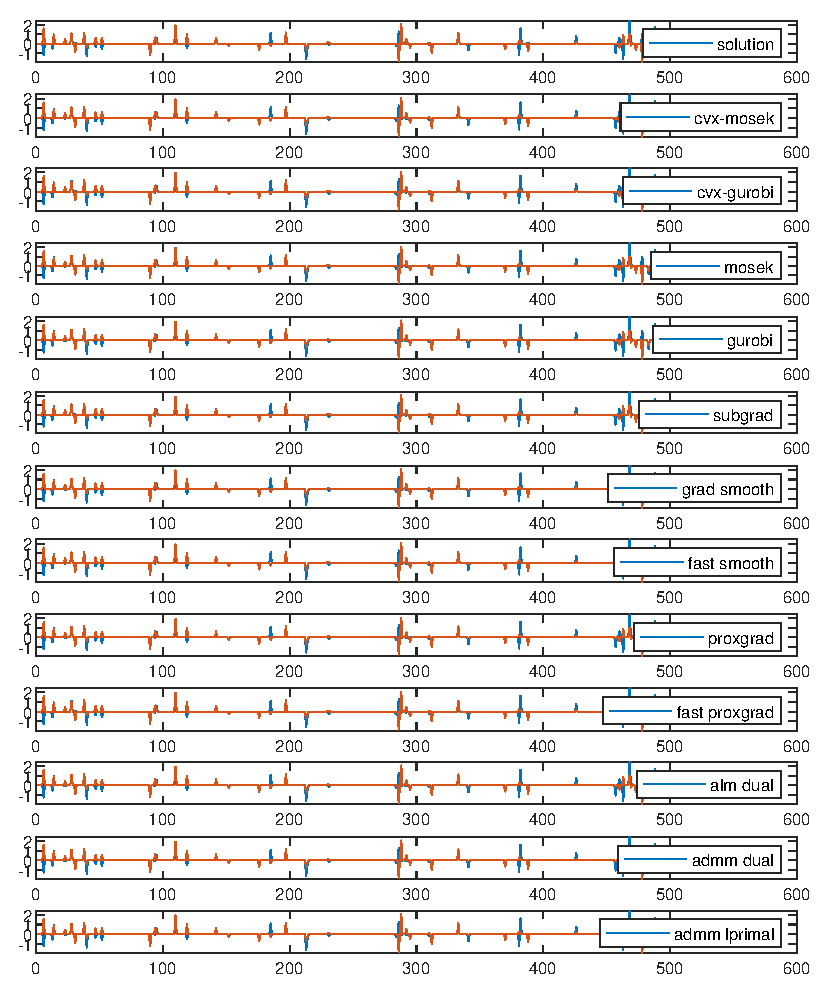
\includegraphics[width=\textwidth]{hw.eps}
    \caption{Visualization of solutions. $l=2$.}
    \label{fig:my_label}
\end{figure}



% \bibliographystyle{plain}
% \bibliography{bib.bib}

\end{document}
